% !TeX encoding=utf8
% !TeX spellcheck = en-US
\documentclass[a4paper]{book}

\usepackage[htt]{hyphenat}
\usepackage[NoDate]{currvita}
\usepackage{parskip}
\usepackage{epstopdf}
\usepackage{graphicx}
\usepackage{tabularx}
\usepackage{booktabs}
\usepackage{lineno,hyperref}
\usepackage{float}
\usepackage{array}
\usepackage{amsmath}
\usepackage[T1]{fontenc}
\usepackage[utf8]{inputenc}
\usepackage{textcomp}
\usepackage{float}
\usepackage{caption}
\usepackage{subcaption}
\usepackage{color}
\usepackage{listings}
\usepackage{color}
\usepackage{url}
\usepackage{dcolumn}
\usepackage{gensymb}
\usepackage{pdflscape}
\usepackage{bbding}
\usepackage{rotating}
\usepackage{caption}
\captionsetup[lstlisting]{singlelinecheck=off}
\usepackage{amssymb}
\usepackage{gensymb}
\usepackage[chapter]{algorithm}
\usepackage{algorithmicx}
\usepackage{algpseudocode}
\usepackage{epstopdf}
\usepackage{tikz,ifthen,xstring,calc,pgf,pgfkeys,pgfopts,pgffor,pgfmath}
\usetikzlibrary{matrix,chains,positioning,decorations.pathreplacing,arrows}
\usepackage{array}
\usepackage{enumitem}

\raggedbottom


% From https://tex.stackexchange.com/questions/83882/how-to-highlight-python-syntax-in-latex-listings-lstinputlistings-command 
% Default fixed font does not support bold face

% Custom colors
\definecolor{deepblue}{rgb}{0,0,0.5}
\definecolor{deepred}{rgb}{0.6,0,0}
\definecolor{deepgreen}{rgb}{0,0.5,0}
\definecolor{gray}{rgb}{0.4, 0.4, 0.4}

% Python style for highlighting
\newcommand\pythonstyle{\lstset{
language=Python,
basicstyle=\footnotesize\ttfamily,
otherkeywords={self},
keywordstyle=\color{deepblue},
emphstyle=\color{deepred},
stringstyle=\color{deepgreen},
commentstyle=\color{gray},
numbers=left,
frame=single,
showstringspaces=false            % 
}}

% Python environment
\lstnewenvironment{python}[1][]
{
\pythonstyle
\lstset{#1}
}
{}

% Python for external files
\newcommand\pythonexternal[2][]{{
\pythonstyle
\lstinputlisting[#1]{#2}}}

% Python for inline
\newcommand\pythoninline[1]{{\pythonstyle\lstinline!#1!}}




% Custom colors
\definecolor{deepblue}{rgb}{0,0,0.5}
\definecolor{deepred}{rgb}{0.6,0,0}
\definecolor{deepgreen}{rgb}{0,0.5,0}
\definecolor{gray}{rgb}{0.4, 0.4, 0.4}

% MATLAB style for highlighting
\newcommand\matlabstyle{\lstset{
    language=MATLAB,%
    basicstyle=\footnotesize\ttfamily,
    morekeywords={matlab2tikz},
    keywordstyle=\color{deepblue},%
    morekeywords=[2]{1}, keywordstyle=[2]{\color{black}},
    identifierstyle=\color{black},%
    stringstyle=\color{deepgreen},
    commentstyle=\color{gray},%
    showstringspaces=false,%without this there will be a symbol in the places where there is a space
    numbers=left,%
    frame=single,
    emph=[1]{for,end,break},emphstyle=[1]\color{red} %some words to emphasise
}}

% MATLAB environment
\lstnewenvironment{matlab}[1][]
{
\matlabstyle
\lstset{#1}
}
{}

% MATLAB for external files
\newcommand\matlabexternal[2][]{{
\matlabstyle
\lstinputlisting[#1]{#2}}}

% MATLAB for inline
\newcommand\matlabinline[1]{{\matlabstyle\lstinline!#1!}}



% Use Biber for citations:
\usepackage[
  style=alphabetic,
  natbib=true,
  backend=biber,
  bibwarn=true,
  texencoding=utf-8,
  bibencoding=utf-8,
]{biblatex} 
\addbibresource{bib/bibtex.bib}
\title{PyThesis - A Python Framework for \LaTeX}
\author{Henning Metzmacher}
\begin{document}
\maketitle
\clearpage
\thispagestyle{empty}
\section*{Abstract}
PyThesis is a lightweight Python framework that lets you integrate Python code into \LaTeX documents. The framework consists of two components: A web React application that can be used to quickly build and view the final PDF document and a Python backend that acts as a preprocessor for the \LaTeX code and embedded Python code. The framwork also contains classes that can be used to interact with a shared MathWorks MATLAB session. Specifically, datasets can be loaded using the Python CSV loader and then sent to MATLAB for further processing or to generate plots. The resulting graphics can be stored in a predefined directory in order to directly embed them as \LaTeX figures.
\clearpage
\tableofcontents
\chapter{Setup}
\label{ch:setup}
\section{Install \LaTeX}
In order to compile \LaTeX files, a \LaTeX distribution needs to be installed. PyThesis executes pdflatex to generate a PDF file after transpiling the source files. For Windows, the proTeXt distribution is recommended: \url{https://www.tug.org/protext/}

\section{Install Python Dependencies}
The software was tested using Python 3.6. Installation using pip: 
\begin{verbatim}
pip install numpy
pip install matplotlib
pip install jinja2
pip install flask
pip install flask_cors
\end{verbatim}
In Linux use pip3 instead.
\section{Install npm to modify the Browser App (Optional)}

\textbf{The prebuild app is now part of the repository. You can skip this unless you want to modify the app}

The browser app is written using the React framework. Node.js needs to be installed to generate a build: \url{https://nodejs.org} 
\begin{verbatim}
cd app
npm install
npm run build
\end{verbatim}
This generates a static build that is served by the integrated Python Flask server.  
\section{Install the MATLAB Engine API for Python (Optional)}
Follow the Mathworks tutorial: \url{https://de.mathworks.com/help/matlab/matlab_external/install-the-matlab-engine-for-python.html}

\section{Run PyThesis}
In Windows you can click on the run\_example.bat to start the example. The webapp should open in a new browser window. Using the command line, the software can be started as follows: 
\begin{verbatim}
python start.py --project_root <project_root>
\end{verbatim}
On Linux use python3 instead. <project\_root> should be replaced with an absolute project path. In order to test the framework and the browser app point <project\_root> to the example project. A new project should match the layout of the example.


\section{Build}
\label{sec:build}
In order to \textbf{build} the document press \textbf{b} or click the play button in the web app. This executes all .py files and generates .tex files from them, merges them into one output document in the build directory and compiles it using the pdflatex (the exact order of build commands is defined in the build.config in the PyThesis root directory, each line is a single command). At some point, when the project grows bigger you might only want to build specific files that you are working on at the moment. In order to that you can do a \textbf{partial build} by pressing \textbf{p}.  

\subsection{\_.always Files}
During a \textbf{partial build} only .py files listed in an \_.always file in that same directory are executed. All other .py files are ignored during a \textbf{partial build}. If, for example, the examples folder contains an \_.always file with a single entry: 
\begin{verbatim}
a_simple_text_generator
\end{verbatim}
this means a\_simple\_text\_generator.py is always executed during a \textbf{partial build} (during a full build it is executed no matter what). The .py extension is automatically appended. In order to add multiple entries just add them in new lines like so:
\begin{verbatim}
file1
file2
etc
\end{verbatim}
In addition, you can do a \textbf{partial execute} by pressing \textbf{e} which is the same as a \textbf{partial build} just that the subsequent \LaTeX build step is omitted. Hence, you won't see updates in the document. 

Python output is always shown in the console (for example the command prompt in Windows).

Table \ref{tab:shortcuts} shows an overview over the build shortcuts in the web application:
\begin{table}[H]
\begin{center}
\begin{tabular}{l|l}
\toprule
Shortcut & Command \\
\midrule
\textbf{b} & \textbf{Full build} (execute all .py files + compilation) \\
\textbf{p} & \textbf{Partial build} (execute only .py files listed in \_.always files + compilation) \\
\textbf{e} & \textbf{Partial execute} (execute only .py files listed in \_.always files) \\
\bottomrule
\end{tabular}
\caption{Overview over the build shortcuts in the web application}
\label{tab:shortcuts}
\end{center}
\end{table}
\chapter{Overview of the API}
\label{ch:overview-of-the-api}
\section{Folder Structure}
\label{sec:folder-structure}
PyThesis uses the following for a project:
\begin{verbatim}
build/ 
data/
src/
templates/
\end{verbatim}
\textbf{build} stores the combined, transpiled tex file as well as \LaTeX output files such as the generated PDF. \textbf{data} should hold CSV files that can be loaded using the Dataset class or \_matlab. \textbf{src} should store all \LaTeX and Python source files. \\

\textbf{NOTE: DO NOT EDIT SOURCE FILES IN THE build FOLDER. THEY WILL GET OVERWRITTEN. ALSO .tex FILES IN \_tex FOLDERS UNDER src ARE OVERWRITTEN.} \\

The \emph{templates} folder should contain reusable templates along with their default JSON files.
\section{Globals}
\label{sec:globals}
PyThesis provides the following global variables when executing the .py files in a project:
\begin{verbatim}
_matlab     Instance of the MatlabAdapter class
_templater  Instance of the Templater class 
_project    Current project root path
_data       Current data path 
_build      Current build path 
_lib        Current lib path (for custom libraries)
_templates  Current templates path 
_file       File path of the executing .py file 
_dir        Containing directory of the executing .py file 
_basename   Basename of the executing .py file 
_name       Name without extension of the executing .py file 
\end{verbatim}

The following modules can be accessed without importing:
\begin{verbatim}
os          Python core library
sys         Python core library
matplotlib  matplotlib module
_plt        matplotlib.pyplot module
np          numpy module
Dataset     PyThesis Dataset class
_dataset    pythesis.dataset module
\end{verbatim}
For an example using \_dataset see the Matplotlib Example, Section \ref{sec:a-matplotlib-plot}.
\section{Jinja}
\label{sec:jinja}
PyThesis uses the Python Jinja templating engine for subincludes and to execute Python code. Therefore Jinja API calls in .tex files have an effect. \LaTeX and Jinja make extensive use of curly brackets so in order to avoid clashes, critical \LaTeX sections can be escape using:
\begin{verbatim}

I can write whatever I want here, nothing gets interpreted.

\end{verbatim}

Jinja documentation: \url{https://jinja.palletsprojects.com/en/2.10.x/}
\section{Subincludes}
\label{sec:subincludes}
PyThesis uses jinja2 and provides a subinclude extension which allows for relative includes. This way LaTeX projects can be structured in much smaller files just like in software projects (there is some native \LaTeX way of doing this but I found this way to be much more convenient). The following example shows a way to organize sub- and subsubsections in a nested fashion. It is of course possible to add further levels, for example, to organize figures and graphics code. The following command includes a tex file which in turn subincludes another tex file:
\begin{verbatim}



\end{verbatim}
The result looks as follows:
\subsection{A Subsection}
\label{sec:a-subsection}
This is a subsection which in turn includes a subsubsection:
\begin{verbatim}



\end{verbatim}
which looks like this:
\subsubsection{A Subsubsection}
\label{sec:a-subsubsection}
This is a subsubsection.
\section{Python Imports}
\label{sec:python-imports}
PyThesis uses the currently executed file as working directory. Modules on the same level can therefore be imported as:
\begin{verbatim}
import _import_me
\end{verbatim}
\textbf{Modules to be imported should be prepended with an underscore}. "Underscored" modules are not compiled directly and do not generate their own .tex files. In order for the imported module to have access to all global variables it needs to be wrapped using the \_wrap function. The \_wrap function also ensures that the module is properly reloaded when the code is changed.
\begin{verbatim}
import _import_me
_wrap(_import_me)
\end{verbatim}
Import example:
\begin{verbatim}
Hello Import. I am imported by imports.py
\end{verbatim}
\chapter{Examples}
\label{ch:examples}

\section{A Simple Text Generator}
\label{sec:a-simple-text-generator}
The text below is generated by the following code:
\begin{python}
sentence = 'Sphinx of black quartz, judge my vow'
for i in range(1, len(sentence) + 1):
    print(f'{sentence[:i]}\\\\')

\end{python}
S\\
Sp\\
Sph\\
Sphi\\
Sphin\\
Sphinx\\
Sphinx \\
Sphinx o\\
Sphinx of\\
Sphinx of \\
Sphinx of b\\
Sphinx of bl\\
Sphinx of bla\\
Sphinx of blac\\
Sphinx of black\\
Sphinx of black \\
Sphinx of black q\\
Sphinx of black qu\\
Sphinx of black qua\\
Sphinx of black quar\\
Sphinx of black quart\\
Sphinx of black quartz\\
Sphinx of black quartz,\\
Sphinx of black quartz, \\
Sphinx of black quartz, j\\
Sphinx of black quartz, ju\\
Sphinx of black quartz, jud\\
Sphinx of black quartz, judg\\
Sphinx of black quartz, judge\\
Sphinx of black quartz, judge \\
Sphinx of black quartz, judge m\\
Sphinx of black quartz, judge my\\
Sphinx of black quartz, judge my \\
Sphinx of black quartz, judge my v\\
Sphinx of black quartz, judge my vo\\
Sphinx of black quartz, judge my vow\\
\section{A Matplotlib Plot}
\label{sec:a-matplotlib-plot}
Python files should be created within a directory called \textbf{py} on the level of the including .tex file. The transpiler creates a folder named \textbf{\_tex} on the same level as the py folder. This folder includes resulting .tex files on the level of the including .tex file. Hence, if on the level of this file there is a directory as follows:
\begin{verbatim}
py/a_matplotlib_plot.py
\end{verbatim}
then the result can be embedded using:
 % This is necessary so that the example subinclude is not interpreted (remember, this gets done in Python BEFORE it reaches the LaTeX compiler) 
\begin{verbatim}

\end{verbatim}

The .tex extension is added automatically. In order to execute Python code to plot or generate illustrations you can use global variables that point to respective project paths. In addition, you can use global objects and classes that can be used to perform common tasks like data set loading. The following is used to create Figure \ref{fig:a_matplotlib_plot}.
% Use the defined python listing style:
\begin{python}
columns = [
    {'key': 'SECONDS'},
    {'key': 'T_01'},
    {'key': 'T_02'}
]
csv_file = f'{_data}/example.csv'
dataset = _dataset.load_dataset(csv_file, columns)
data = dataset.to_dict()
fig, ax = _plt.subplots(figsize=(6, 4))
ax.plot(data['SECONDS'], data['T_01'])
ax.plot(data['SECONDS'], data['T_02'])
ax.set(
    xlabel='Time [s]',
    ylabel='Temperature [\u00b0C]',
    title='A Matplotlib Plot',
    ylim=[30, 40]
)
ax.legend(['Temperature 1', 'Temperature 2'])
ax.grid()
_plt.tight_layout()
fig.savefig(f'{_build}/images/{_name}.pdf')
figure = _templater.render(
    f'{_templates}/latex/figure.tex',
    path=f'images/{_name}',
    label=f'fig:{_name}',
    caption='A Matplotlib Plot'
)
print(figure)

\end{python}
\begin{figure}[H]
\begin{center}
  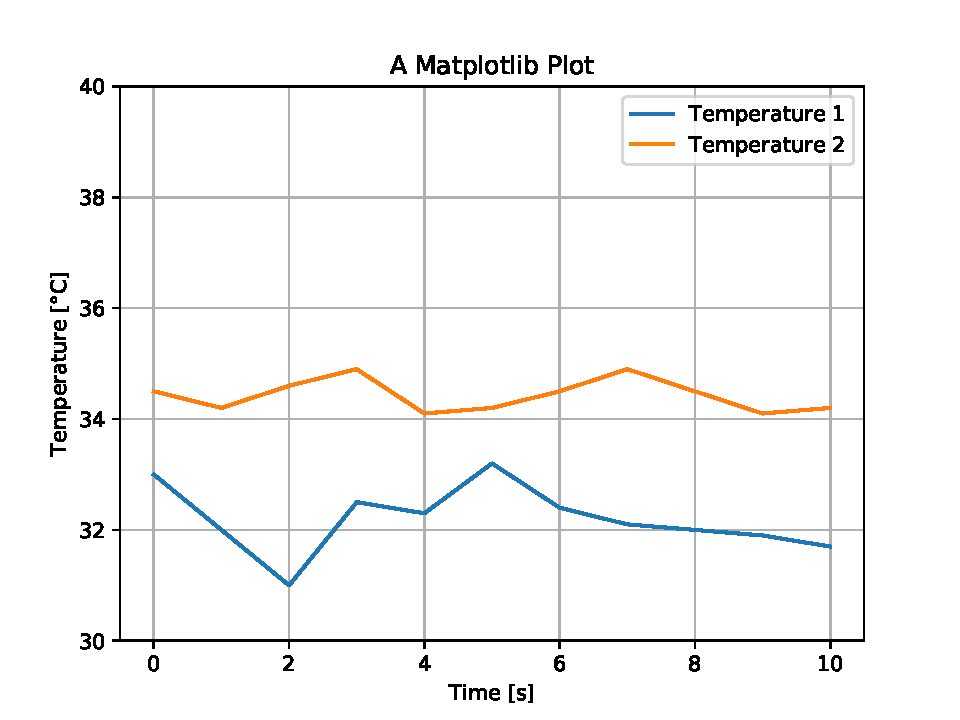
\includegraphics[width=\textwidth]{images/a_matplotlib_plot}
  \caption{A Matplotlib Plot}
  \label{fig:a_matplotlib_plot}
\end{center}
\end{figure}
\section{A MATLAB Plot}
\label{sec:a-matlab-plot}
In order to generate MATLAB plots PyThesis needs to be started with the MATLAB flag:
\begin{verbatim}
python start.py [...] --matlab
\end{verbatim}
The MATLAB Python engine must be installed and MATLAB must be running. In order to share the MATLAB engine, enter the following command into the MATLAB terminal:
\begin{verbatim}
matlab.engine.shareEngine
\end{verbatim}
The following uses the \_matlab singleton, the \_templater and \_dataset to generate a MATLAB plot:  
\begin{python}
# Only execute if the _matlab singleton exists:
if not(_matlab == None):
    columns = [
        {'key': 'SECONDS'},
        {'key': 'T_01'},
        {'key': 'T_02'}
    ]
    _matlab.load_dataset(f'{_data}/example.csv', _name, columns)
    _matlab.eval_template(
        f'{_templates}/matlab/figure.m',
        height=300
    )
    _matlab.eval_template(
        './a_matlab_plot.m',
        name=_name
    )
    _matlab.eval_template(
        f'{_templates}/matlab/axis.m',
        xlabel='Time [s]',
        ylabel='Temperature [\u00b0C]',
        xmin=0,
        xmax=10,
        xtickminor=1,
        xtick=5,
        ymin=30,
        ymax=40,
        ytickminor=1,
        ytick=5
    )
    _matlab.eval_template(
        f'{_templates}/matlab/pdf.m',
        pdfpath=f'{_build}/images/{_name}.pdf'
    )
figure = _templater.render(
    f'{_templates}/latex/figure.tex',
    label=f'fig:{_name}',
    caption='A MATLAB Plot',
    path=f'images/{_name}'
)
print(figure)

\end{python}
The following shows the accompanying MATLAB template "a\_matlab\_plot.m". Note that the variable "name" within the double curly brackets is replaced with the parameter set in eval\_template in the .py script above (for information on Jinja templates see Section \ref{sec:jinja}).

\begin{matlab}
hold on;
p1 = plot( ...
    {{name}}.SECONDS, ...
    {{name}}.T_01, ...
    'Color', 'k',  ...
    'LineWidth', 1 ...
);
p2 = plot( ...
    {{name}}.SECONDS, ...
    {{name}}.T_02, ...
    '--', ...
    'Color', 'k', ...
    'LineWidth', 1 ...
);
title('A MATLAB Plot');
legend([p1, p2], 'Temperature 1', 'Temperature 2');
hold off

\end{matlab}

\begin{figure}[H]
\begin{center}
  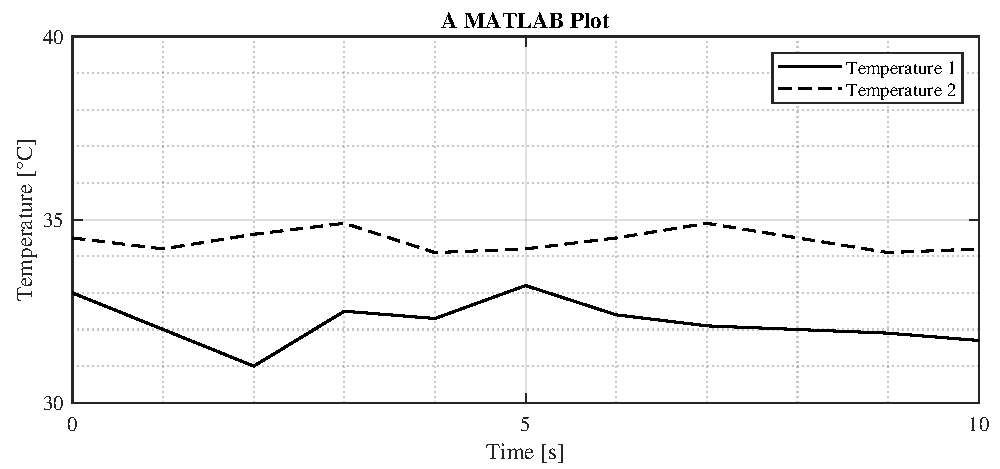
\includegraphics[width=\textwidth]{images/a_matlab_plot}
  \caption{A MATLAB Plot}
  \label{fig:a_matlab_plot}
\end{center}
\end{figure}
\section{A Table}
\label{sec:a-table}
This example shows how to load a CSV file into a dataset and display it as a table. In addition, the dataset metrics function can be used to calculate statistical metrics from the data and append it to the table.
\begin{table}[H]
\begin{center}
\begin{tabular}{c|cc}
\toprule
Seconds/Metric & T\_01 & T\_02 \\
\midrule
0.0 & 33.0 & 34.5 \\ 
1.0 & 32.0 & 34.2 \\ 
2.0 & 31.0 & 34.6 \\ 
3.0 & 32.5 & 34.9 \\ 
4.0 & 32.3 & 34.1 \\ 
5.0 & 33.2 & 34.2 \\ 
6.0 & 32.4 & 34.5 \\ 
7.0 & 32.1 & 34.9 \\ 
9.0 & 31.9 & 34.1 \\ 
10.0 & 31.7 & 34.2 \\ 
\midrule 
\mu & 32.21 & 34.42 \\ 
\sigma & 0.6 & 0.29 \\ 
median & 32.2 & 34.35 \\ 
min & 31.0 & 34.1 \\ 
max & 33.2 & 34.9 \\
\bottomrule
\end{tabular}
\end{center}
\caption{A table example}
\label{tab:a-table-example}
\end{table}

Python code to generate the table:
\begin{python}
rows = []
columns = [
    {'key': 'SECONDS'},
    {'key': 'T_01'},
    {'key': 'T_02'}
]
dataset = _dataset.load_dataset(
    f'{_data}/example.csv', 
    columns=columns
)

# Extract a matrix and the metrics from the dataset:
matrix = dataset.to_matrix(['SECONDS', 'T_01', 'T_02'])
metrics = dataset.metrics(['T_01', 'T_02'])

# Create LaTeX table rows from values:
for row in matrix:
    rows.append(' & '.join(map(str, row)) + ' \\\\')

# Add a line between the values and the metrics:
rows.append('\\midrule')

# Map values to strings so we can join them:
means   = map(str, metrics['mean'])
stds    = map(str, metrics['std'])
medians = map(str, metrics['median'])
mins    = map(str, metrics['min'])
maxs    = map(str, metrics['max'])

# Create LaTex table rows from metrics:
rows.append('\mu & '    + ' & '.join(means)   + ' \\\\')
rows.append('\sigma & ' + ' & '.join(stds)    + ' \\\\')
rows.append('median & ' + ' & '.join(medians) + ' \\\\')
rows.append('min & '    + ' & '.join(mins)    + ' \\\\')
rows.append('max & '    + ' & '.join(maxs)    + ' \\\\')

# Render the table:
table = _templater.render(
    f'./a_table.tex',
    rows=' \n'.join(rows),
    name=f'a_table'
)
print(table)

\end{python}
\section{Custom Library}
\label{sec:custom-library}
This example shows how to create a custom class in the lib directory and use it to create Matplotlib plots.
\begin{figure}[H]
\begin{center}
  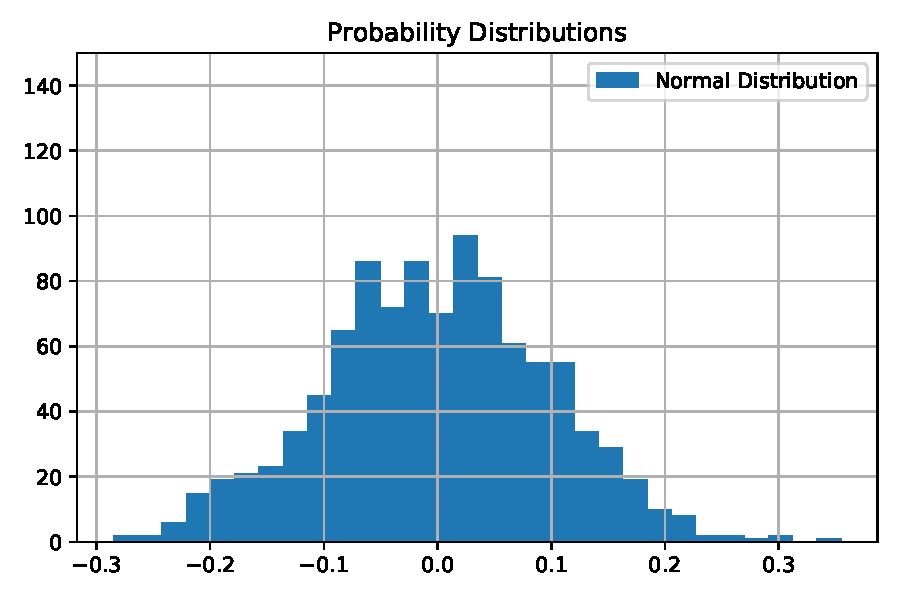
\includegraphics[width=\textwidth]{images/normal}
  \caption{Normal Distribution}
  \label{fig:normal}
\end{center}
\end{figure}
\begin{figure}[H]
\begin{center}
  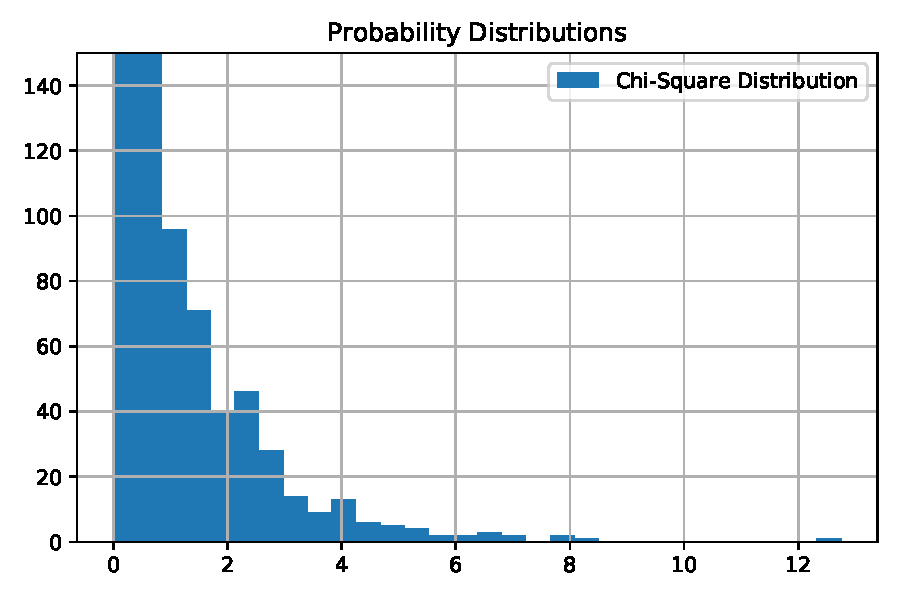
\includegraphics[width=\textwidth]{images/chisquare}
  \caption{Chi-Square Distribution}
  \label{fig:chisquare}
\end{center}
\end{figure}
Distribution classes used in the example (in module lib/\_distributions):
\begin{python}
class NormalDistribution:
    def __init__(self, mu=0, sigma=0.1):
        self.mu = mu
        self.sigma = sigma
   
    def generate_samples(self, num_samples=1000):
        return _np.random.normal(self.mu, self.sigma, num_samples)

class ChiSquareDistribution:
    def __init__(self, df=1):
        self.df = df

    def generate_samples(self, num_samples=1000):
        return _np.random.chisquare(self.df, num_samples)

\end{python}
Plot code:
\begin{python}
sys.path.append(_lib) # Manually add _lib to system path
# The leading underscore of the _distribution module is only 
# by convention and not technically necessary. However, it 
# helps to keep the code clutter free especially when using 
# short, precise module names that might also be used as 
# variable names (without the leading underscore):
import _distributions
# Reload the module manually to include latest changes: 
importlib.reload(_distributions)
# In order for lib modules to have access to project globals 
# they also need to be wrapped:
_wrap(_distributions)

def plot_histogram(samples, label, name):
    fig, ax = _plt.subplots(figsize=(6, 4))
    ax.hist(samples, bins=30)
    ax.set(title='Probability Distributions', ylim=[0, 150])
    ax.legend([label])
    ax.grid()
    _plt.tight_layout()
    fig.savefig(f'{_build}/images/{name}.pdf')
    figure = _templater.render(
        f'{_templates}/latex/figure.tex',
        path=f'images/{name}',
        label=f'fig:{name}',
        caption=label
    )
    print(figure)

# Instantiate the distribution classes:
normal_dist         = _distributions.NormalDistribution()
chisquared_dist     = _distributions.ChiSquareDistribution()
# Generate samples:
normal_samples      = normal_dist.generate_samples(1000)
chisquare_samples   = chisquared_dist.generate_samples(1000)
# Set names:
normal_name         = 'Normal Distribution'
chisquare_name      = 'Chi-Square Distribution'
# Plot samples:
plot_histogram(normal_samples, normal_name, 'normal')
plot_histogram(chisquare_samples, chisquare_name, 'chisquare')

\end{python}
\printbibliography
\end{document}